%%% CLASS SETTING %%%
\documentclass[letterpaper, 12pt]{article}
\usepackage{natbib}
\usepackage[margin=1in]{geometry} % sets page layout 
\bibpunct[, ]{(}{)}{,}{a}{}{,} % sets the punctuation of the bibliography entires.

%%% Paper Information %%%
\title{Presenting Analytical Results in \LaTeX} 
\usepackage{authblk} % For Author Affiliation Printing
\author{Gento Kato}
\affil{University of California, Davis}
\date{March 6, 2019}

% Other Packages/Settings
\usepackage{amsfonts, amsmath, amssymb, bm} %Math fonts and symbols
\usepackage[format=hang, justification=centering]{caption}
\usepackage{dcolumn, multirow} % decimal-aligned columns, multi-row cells
\usepackage{graphicx, subfigure, float} % graphics commands
\usepackage{booktabs} % Advanced formatting of table
\usepackage[colorlinks=true, citecolor=blue]{hyperref} % Reference link
\usepackage{setspace}% allows toggling of double/single-spacing
\doublespace % set document spacing to double use \singlespace if you want single space

\begin{document}

    % Set the Style of Bibliography
    \bibliographystyle{apsr}

    \maketitle

    \begin{abstract}
        This sample document describes how you can present R results through \LaTeX.
    \end{abstract}

    \section{Start Using \LaTeX}

    \par \LaTeX generates beautifully formatted PDF file. Different from other text editors such as Word, \LaTeX file must be  \textit{compiled} to obtain the final product (PDF File, most of the time). To write raw \LaTeX files, you need to learn its grammars and rules. While learning curve is somewhat steep, I believe it pays out in the end. In addition to the easy integration with R, it automates formatting and citations, which will save your time when you are reviewing papers. 
    
    \par There are two ways to start using \LaTeX.

    \subsection{Compile Locally}

    \par The standard method to use \LaTeX is to locally compile the file on your own computer. Even when you have no access to internet, this method will give you the power to generate PDF files.

    \begin{enumerate}
        \item Download TeX Distribution -- \href{https://www.tug.org/texlive/acquire-netinstall.html}{TeX Live}, \href{https://miktex.org/download}{MikTeX}, or \href{http://www.tug.org/mactex/mactex-download.html}{MacTeX} (Mac Version of TeX Live) -- to your computer
        \item Install \LaTeX Editor. I would recommend \href{https://www.texstudio.org}{TeX Studio} for the begining user.
        \item Start!
    \end{enumerate}

    \subsection{Compile Online}

    \par Using web-based \LaTeX editor opens up the possibilities by making it possible to share the TeX files without worrying about local dependencies in compilation. Note that, though, if internet is slow or unavailable, you may have stressful time editing documents. The major editor here is \href{https://www.overleaf.com}{Overleaf}. You can just register their and can start editing immediately. Also, their \href{https://www.overleaf.com/learn/latex/Main_Page}{documentation} page is a very rich resource for learning what you can do in \LaTeX.
    
    \subsection{Managing References}
    
    \par Automatic citation is one of the great benefits of using \LaTeX. If you are interested in managing references in \texttt{.bib} or \texttt{.bibtex} format (the format compatible to \LaTeX), you should look for either \href{http://www.jabref.org}{JabRef} or href{https://bibdesk.sourceforge.io}{BibDesk} (Mac Only). Some Reference Managers such as \href{https://www.mendeley.com/?interaction_required=true}{Mendeley} and \href{https://www.zotero.org}{Zotero} have an ability to export reference information in \texttt{.bib} format.

    \section{Dependent Variable}

    \par The dependent variable of interest is \textbf{politicalinterest}. \autoref{dvdist} shows the distribution of this variable.

    \begin{figure}[h!] % t implies top, h implies "here". ! emphasize.
        \centering
          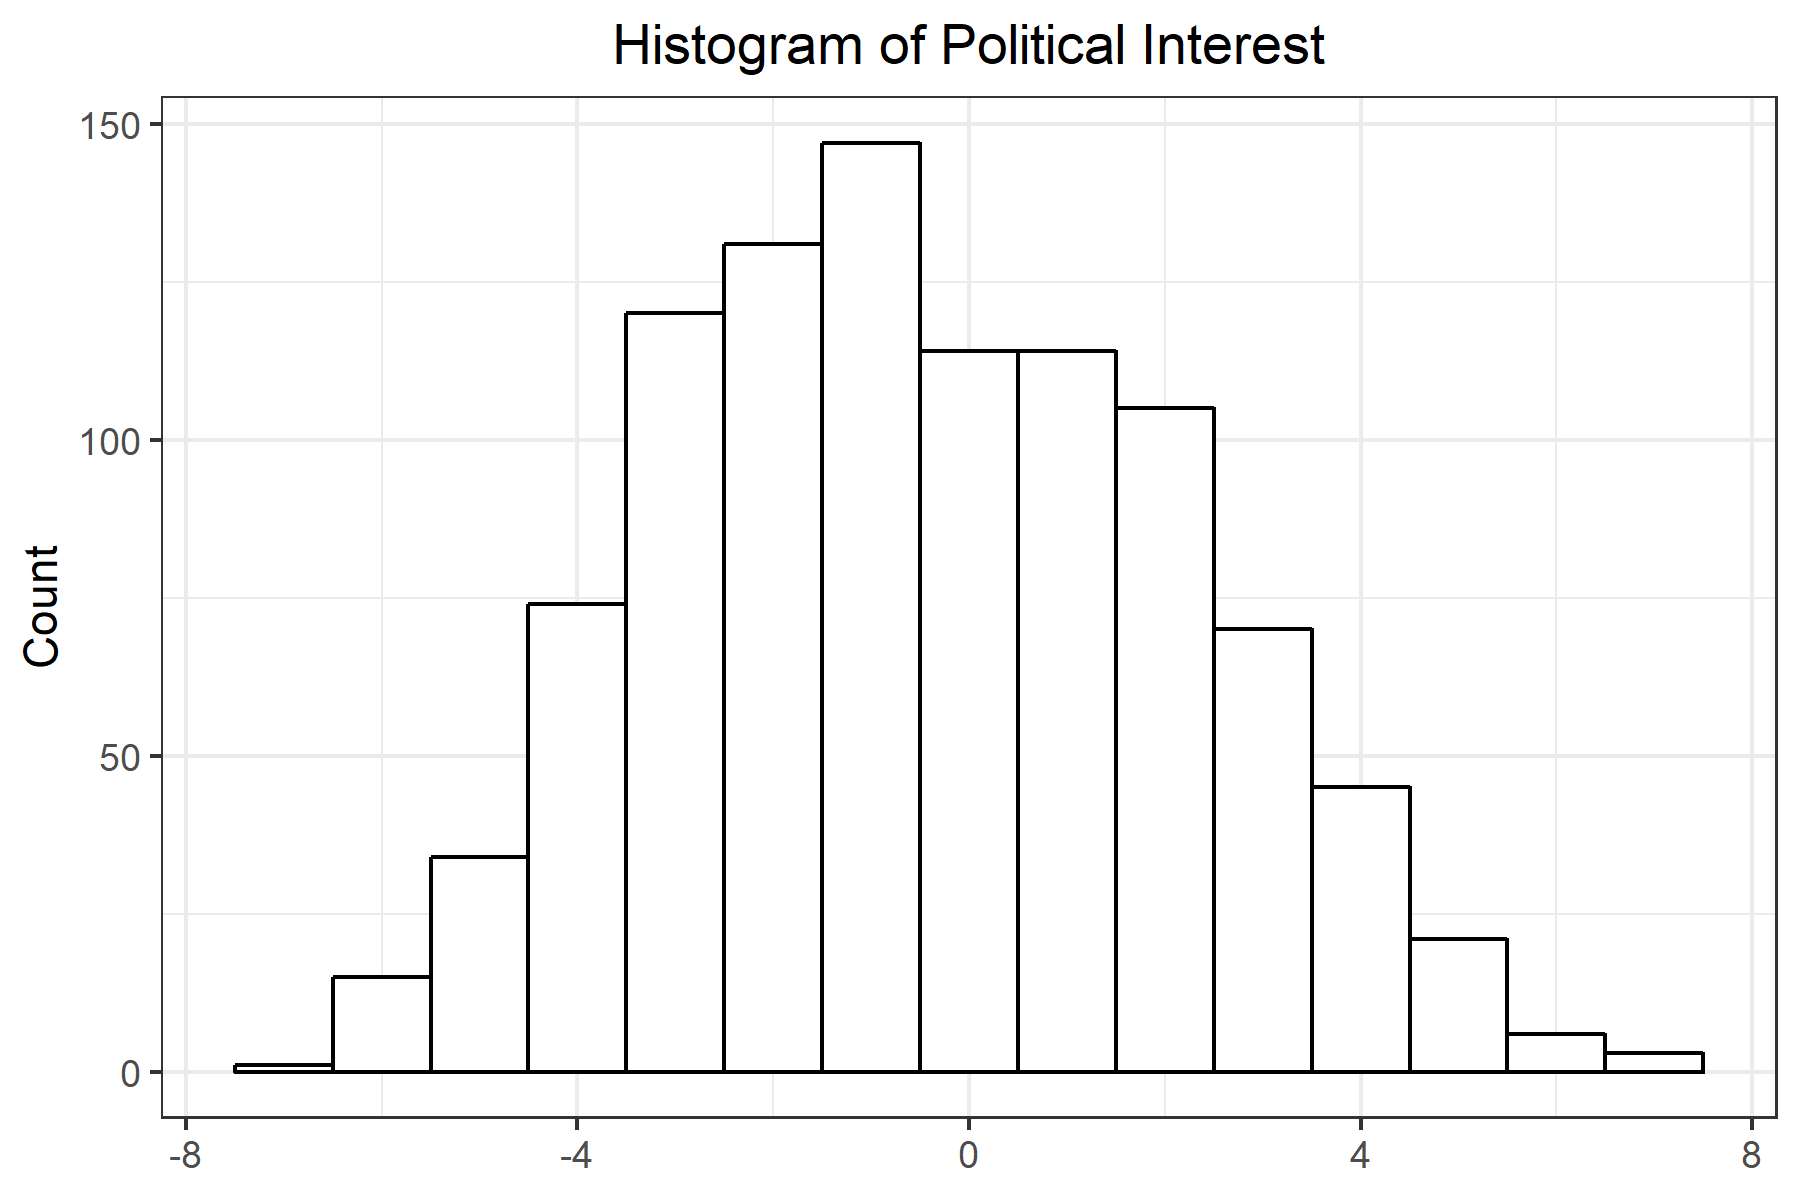
\includegraphics[width=6in]{dvdist.png}
          \caption{Plotted Distribution of Political Interest} %title
          \label{dvdist} %Refer to this graph from texts
    \end{figure}

    \section{Independent Variables}

    \par There are five independent variables. Variables are \textit{age}, \textit{education}, \textit{income}, \textit{female}, and \textit{treatment}. The distributions of those variables are shown in \autoref{ivdist}.

    \begin{figure}[h!] % t implies top, h implies "here". ! emphasize.
        \centering
          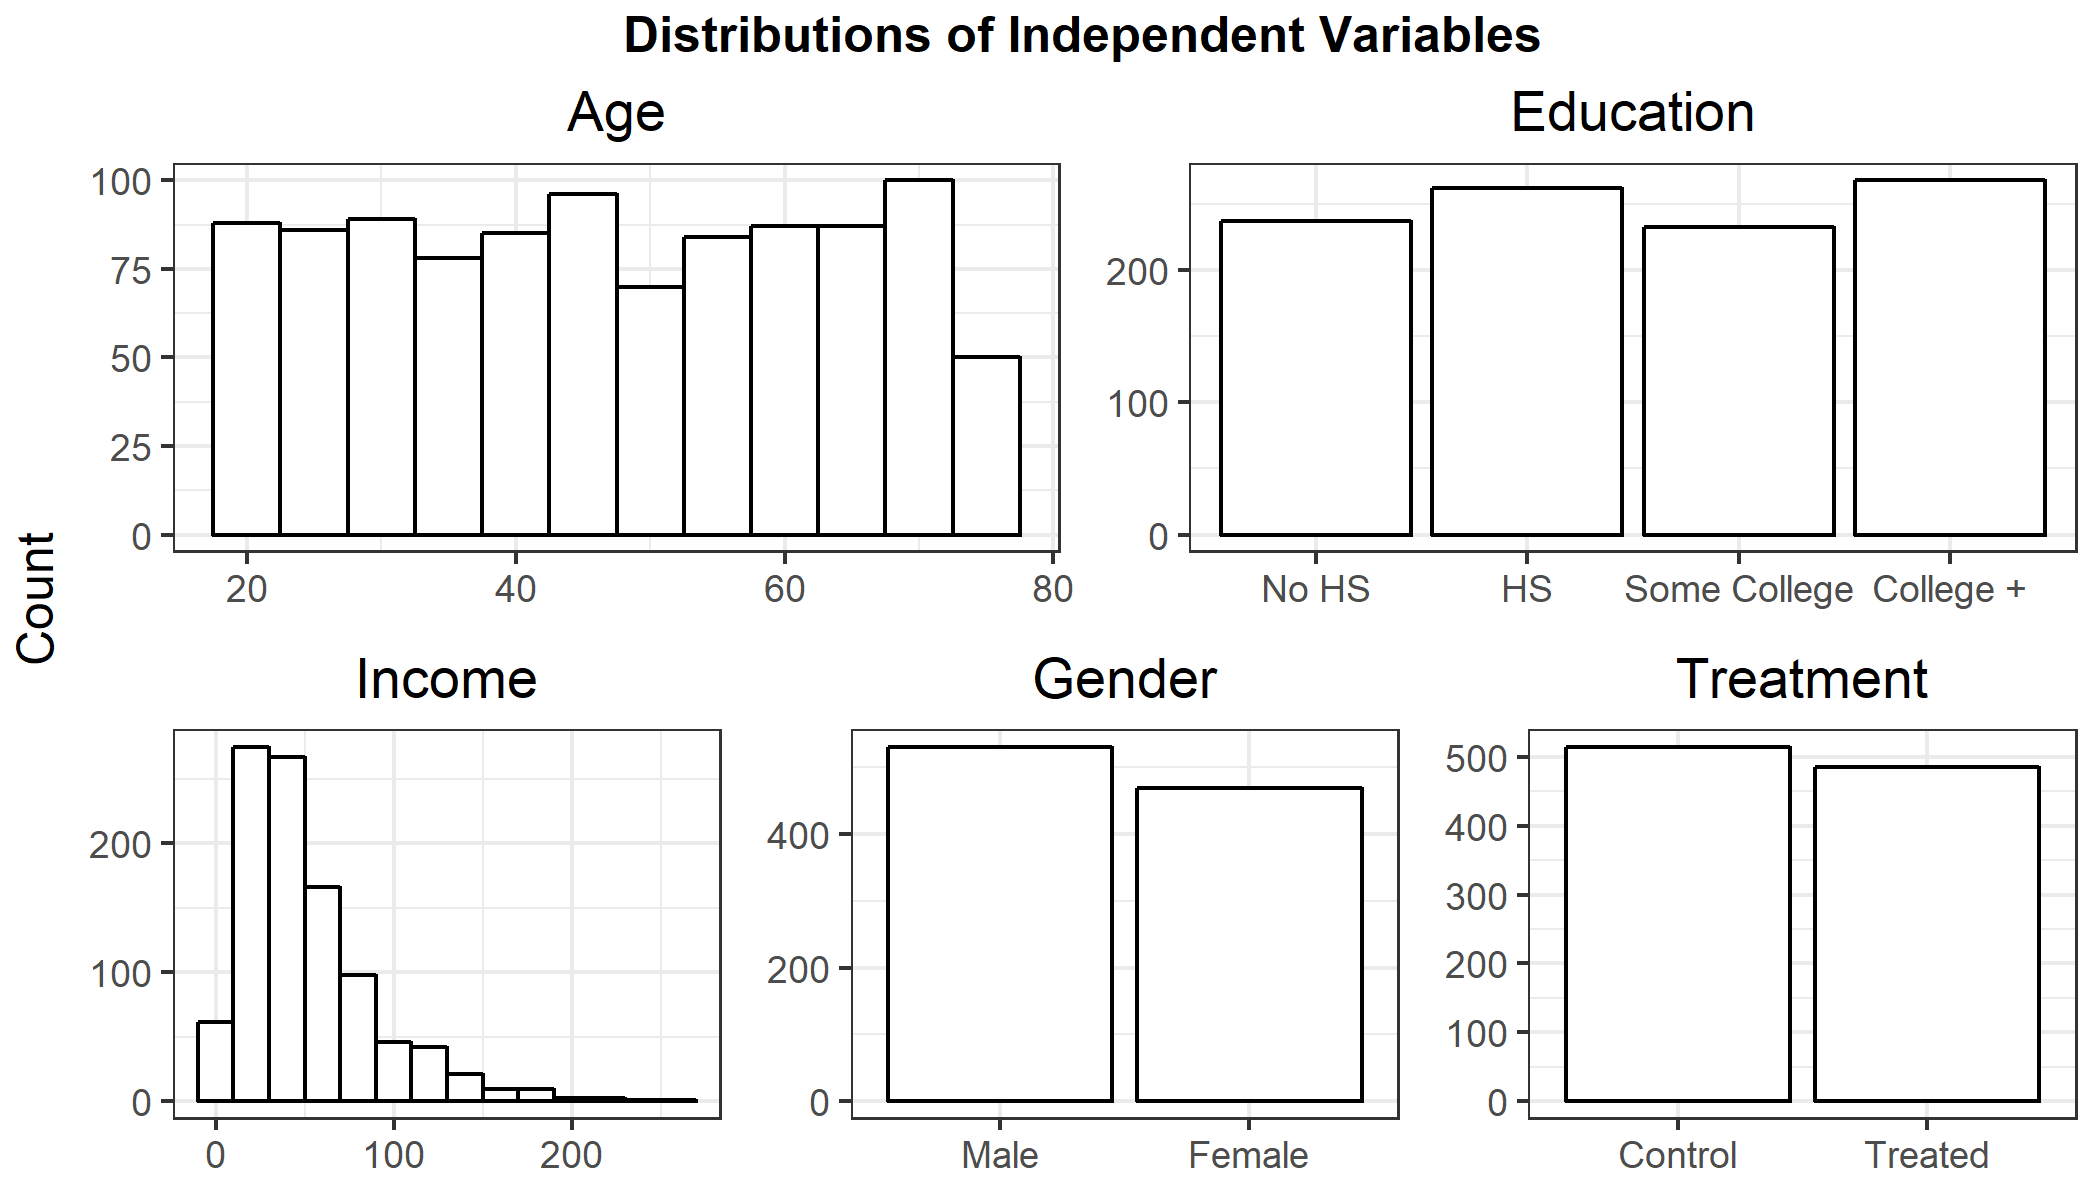
\includegraphics[width=6in]{ivdist.png}
          \caption{Plotted Distribution of Covariates} %title
          \label{ivdist} %Refer to this graph from texts
    \end{figure}

    \clearpage % Go To New Page

    \section{OLS Estimates}

    % Print Table (apsrtable)
    \begin{table}[h!] % t implies top, h implies "here". ! emphasize.
        \centering % center output
        \caption{Multiple Regression Estimates (\texttt{apsrtable})} % title
        \label{apsrtab} % to refer this graph in texts
         
\begin{tabular}{ l D{.}{.}{3}D{.}{.}{3}@{\hspace{2em}}D{.}{.}{3}D{.}{.}{3}@{\hspace{2em}}D{.}{.}{3}D{.}{.}{3} } 
\hline 
  & \multicolumn{ 2 }{ c }{ Model 1 } & \multicolumn{ 2 }{ c }{ Model 2 } & \multicolumn{ 2 }{ c }{ Model 3 } \\ \hline
 (Intercept)              & -9.647 ^*                & (0.247)                  & -11.183 ^*               & (0.269)                  & -9.316 ^*                & (0.244)                 \\ 
Treatment                & 0.460 ^*                 & (0.083)                  & 0.461 ^*                 & (0.088)                  & -0.100                   & (0.111)                 \\ 
Gender (Female)          & 2.483 ^*                 & (0.083)                  & 2.509 ^*                 & (0.088)                  & 1.903 ^*                 & (0.113)                 \\ 
Age                      & 0.050 ^*                 & (0.002)                  & 0.050 ^*                 & (0.003)                  & 0.050 ^*                 & (0.002)                 \\ 
Education (High School)  & 1.168 ^*                 & (0.118)                  &                          &                          & 1.114 ^*                 & (0.115)                 \\ 
Education (Some College) & 1.613 ^*                 & (0.121)                  &                          &                          & 1.575 ^*                 & (0.118)                 \\ 
Education (College/More) & 4.099 ^*                 & (0.117)                  &                          &                          & 4.020 ^*                 & (0.115)                 \\ 
Income (Log)             & 1.009 ^*                 & (0.053)                  & 1.015 ^*                 & (0.056)                  & 1.014 ^*                 & (0.051)                 \\ 
Education (4p Scale)     &                          &                          & 1.292 ^*                 & (0.039)                  &                          &                         \\ 
Treatment * Female       &                          &                          &                          &                          & 1.204 ^*                 & (0.163)                  \\
 $N$        & \multicolumn{2}{c}{1000 } & \multicolumn{2}{c}{1000 } & \multicolumn{2}{c}{1000 }\\ 
$R^2$      & \multicolumn{2}{c}{0.751} & \multicolumn{2}{c}{0.722} & \multicolumn{2}{c}{0.764}\\ 
adj. $R^2$ & \multicolumn{2}{c}{0.749} & \multicolumn{2}{c}{0.720} & \multicolumn{2}{c}{0.762}\\ 
Resid. sd  & \multicolumn{2}{c}{1.311} & \multicolumn{2}{c}{1.383} & \multicolumn{2}{c}{1.277} \\ \hline
 \multicolumn{7}{l}{\footnotesize{Standard errors in parentheses}}\\
\multicolumn{7}{l}{\footnotesize{$^*$ indicates significance at $p< 0.05 $}} 
\end{tabular} 
 % insert table
    \end{table}

    % Print Table (texreg)
    \begin{table}[h!] % t implies top, h implies "here". ! emphasize.
        \centering % center output
        \caption{Multiple Regression Estimates (\texttt{texreg})} % title
        \label{texregtab} % to refer this graph in texts
        
\begin{tabular}{l c c c }
\toprule
 & Model 1 & Model 2 & Model 3 \\
\midrule
(Intercept)              & $-9.65 \; (0.25)^{***}$ & $-11.18 \; (0.27)^{***}$ & $-9.32 \; (0.24)^{***}$ \\
Treatment                & $0.46 \; (0.08)^{***}$  & $0.46 \; (0.09)^{***}$   & $-0.10 \; (0.11)$       \\
Gender (Female)          & $2.48 \; (0.08)^{***}$  & $2.51 \; (0.09)^{***}$   & $1.90 \; (0.11)^{***}$  \\
Treatment * Female       &                         &                          & $1.20 \; (0.16)^{***}$  \\
Age                      & $0.05 \; (0.00)^{***}$  & $0.05 \; (0.00)^{***}$   & $0.05 \; (0.00)^{***}$  \\
Education (High School)  & $1.17 \; (0.12)^{***}$  &                          & $1.11 \; (0.11)^{***}$  \\
Education (Some College) & $1.61 \; (0.12)^{***}$  &                          & $1.58 \; (0.12)^{***}$  \\
Education (College/More) & $4.10 \; (0.12)^{***}$  &                          & $4.02 \; (0.11)^{***}$  \\
Education (4p Scale)     &                         & $1.29 \; (0.04)^{***}$   &                         \\
Income (Log)             & $1.01 \; (0.05)^{***}$  & $1.02 \; (0.06)^{***}$   & $1.01 \; (0.05)^{***}$  \\
\midrule
R$^2$                    & 0.75                    & 0.72                     & 0.76                    \\
Adj. R$^2$               & 0.75                    & 0.72                     & 0.76                    \\
Num. obs.                & 1000                    & 1000                     & 1000                    \\
RMSE                     & 1.31                    & 1.38                     & 1.28                    \\
\bottomrule
\multicolumn{4}{l}{\scriptsize{$^{***}p<0.001$, $^{**}p<0.01$, $^*p<0.05$}}
\end{tabular}
 % insert table
    \end{table}

    % Coefficient Plot
    \begin{figure}[h!] % t implies top, h implies "here". ! emphasize.
        \centering
          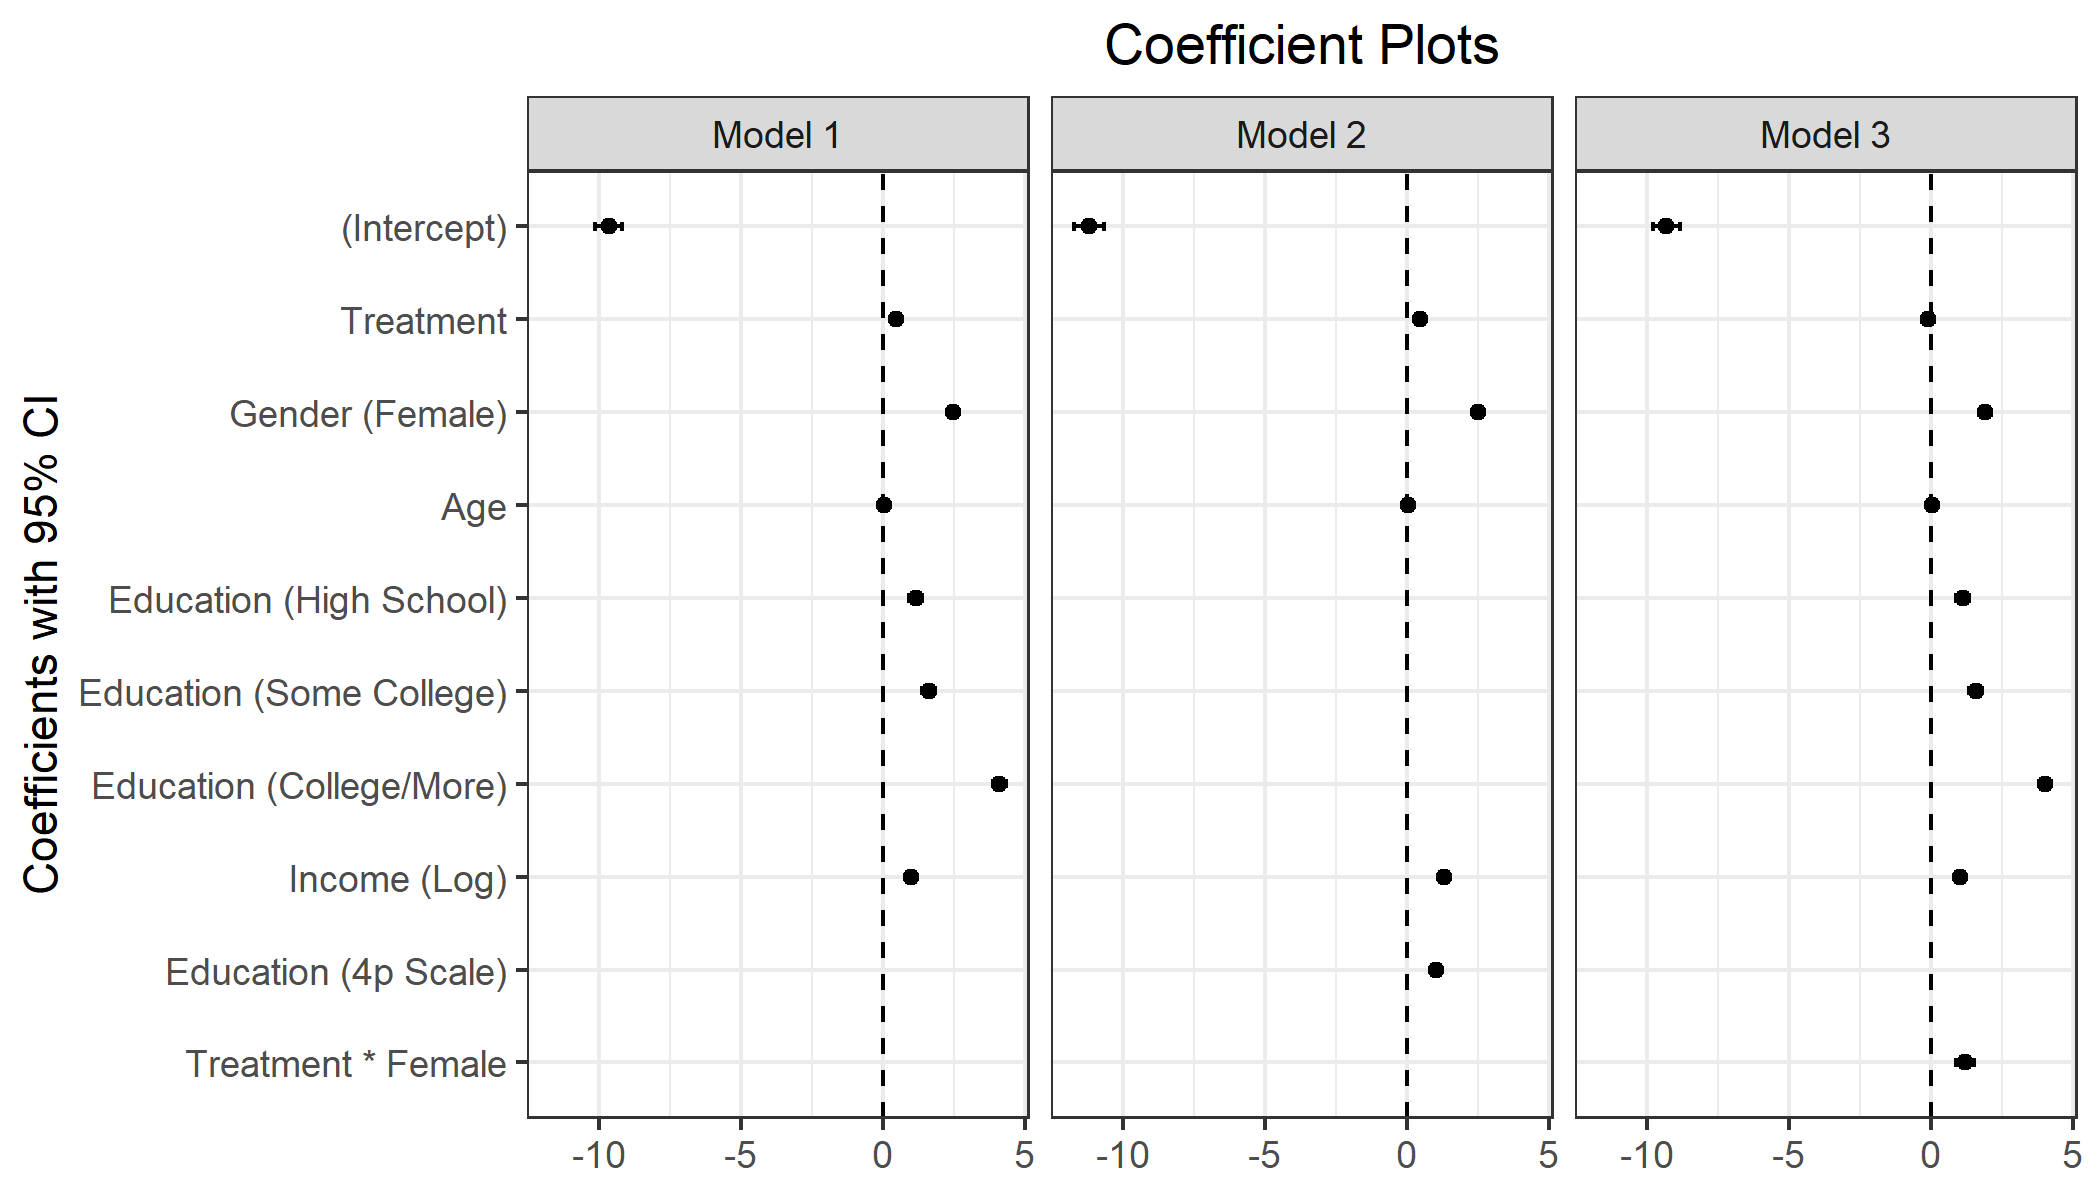
\includegraphics[width=6in]{cp.png}
          \caption{Coefficient Plots} %title
          \label{cp} %Refer to this graph from texts
    \end{figure}


    \section{Interactions}

    % Coefficient Plot
    \begin{figure}[h!] % t implies top, h implies "here". ! emphasize.
        \centering
          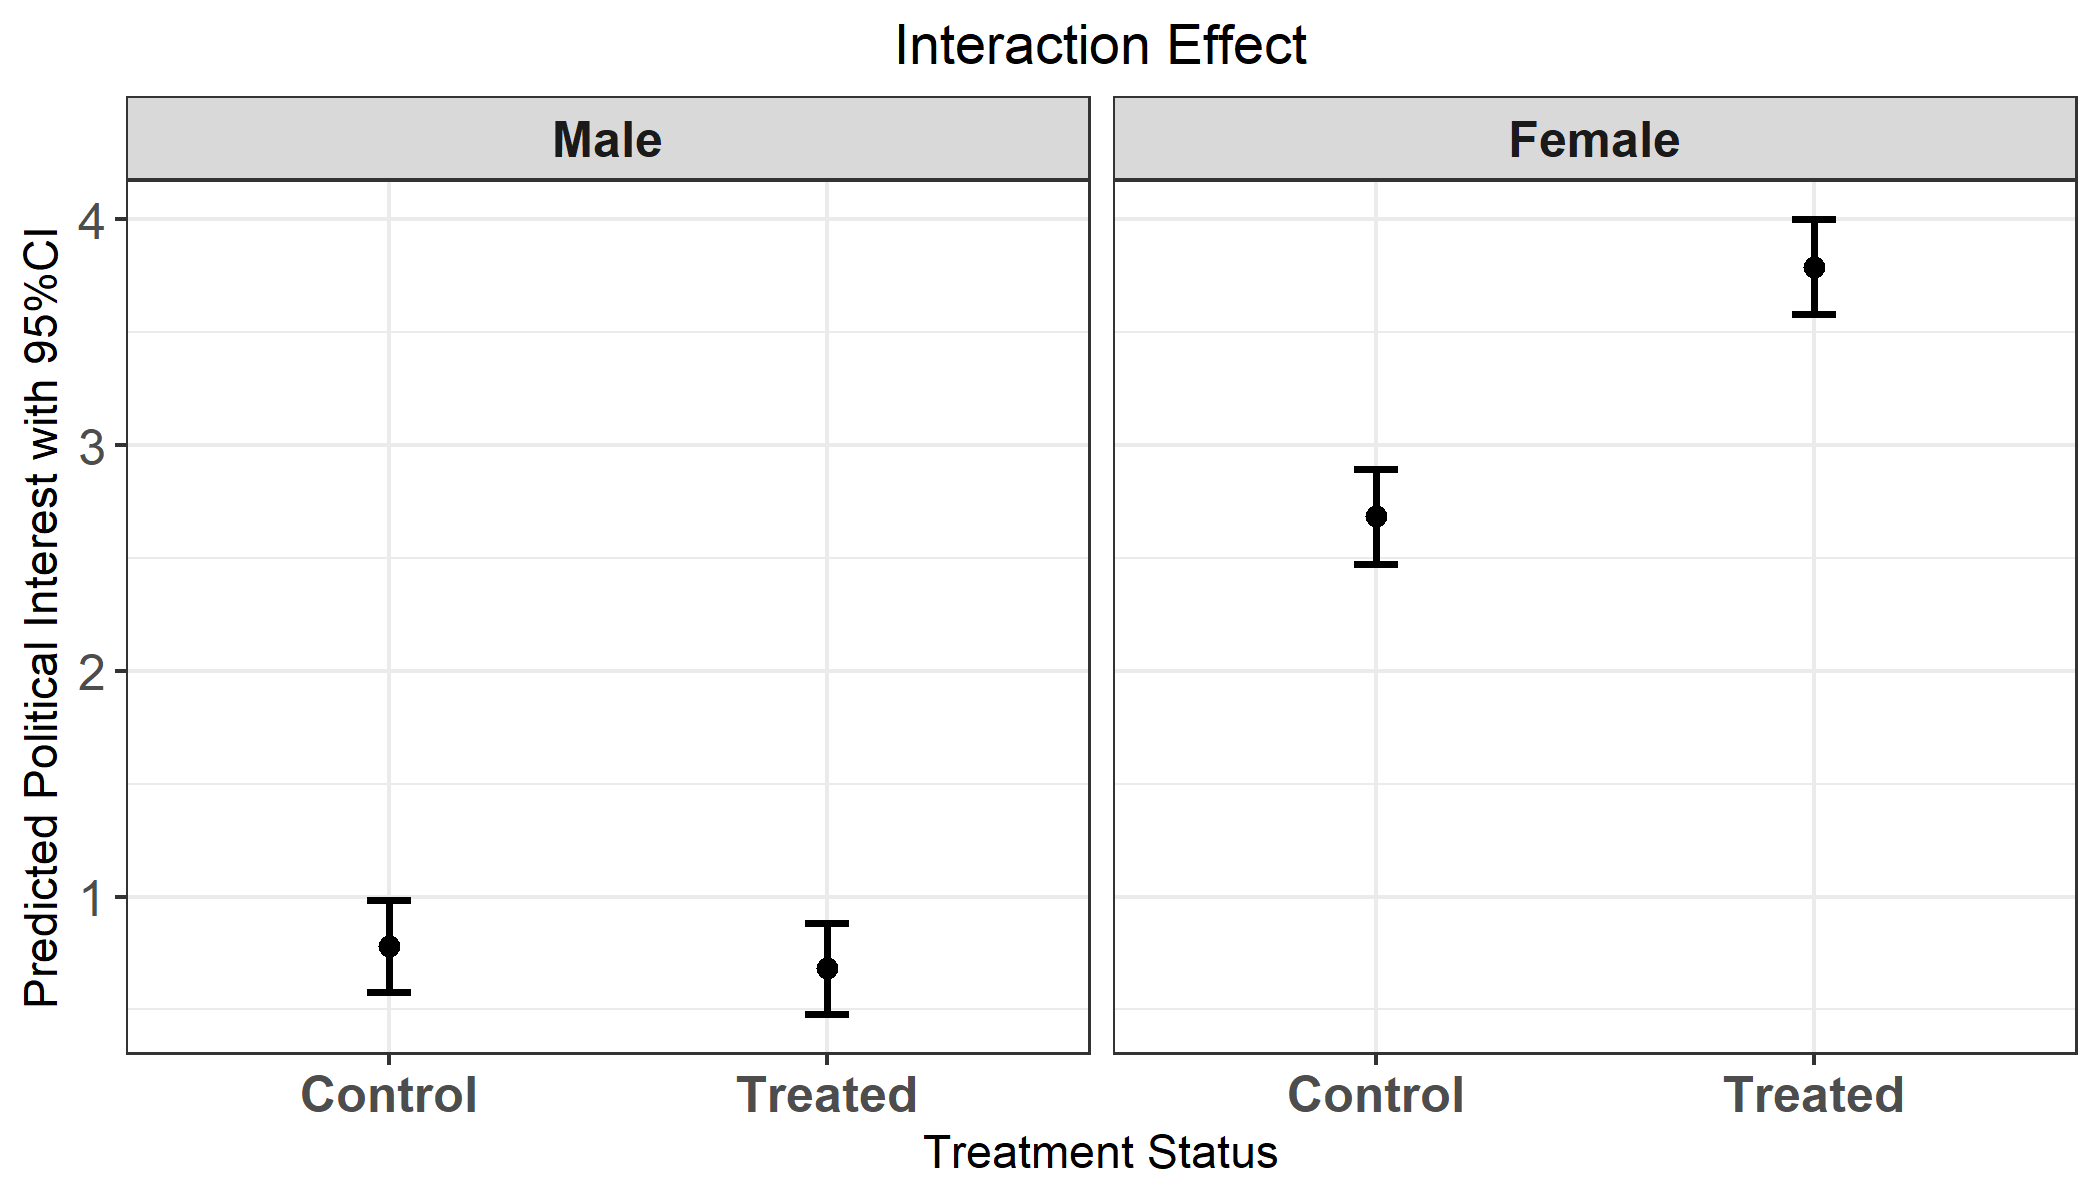
\includegraphics[width=6in]{pri.png}
          \caption{Prediction Plot with Interaction Model} %title
          \label{pri} %Refer to this graph from texts
    \end{figure}

    \par For the interpretation of interacted coefficients, see \cite{Friedrich1982inde} or \cite{Brambor2006unin}. It is also described in the textbook for this class \citep{Fox2016apre}.

    %\clearpage % Add Page Break
    \bibliography{sample.bib}
    
\end{document}